
\documentclass{article}%

\usepackage{amsmath}%
\usepackage{graphicx}
\usepackage[english,greek]{babel}
\usepackage[utf8x]{inputenc}
\usepackage{listings}



\begin{document}

\selectlanguage{greek}

\title{Δίκτυα Επικοινωνιών\\1η εργαστηριακή άσκηση}
\author{Γεώργιος Δασούλας\\Α.Μ: 03112010 \\ 6ο Εξάμηνο 2014-2015  }
\date{24/3/2015}
\maketitle

\textbf{{\underline{1.Το πρώτο \textlatin{Tcl script}
 – Γνωριμία με το \textlatin{NAM} }}}  \\

\textsl{\textbf{Απαντήσεις ερωτήσεων}}
\begin{itemize}
	\item Ποιος είναι ο ρυθμός μετάδοσης σε \textlatin{bit/sec?}\\
	\textbf{Απάντηση} : Από τα δεδομένα το \textlatin{packetsize} ισούται με 1000 \textlatin{bytes} και στέλνεται ένα κάθε 0.005 \textlatin{sec}. Οπότε, ο ρυθμός μετάδοσης $ = \frac{8*1000}{0.005}=1.600.000 $ \textlatin{bits/sec}.
	\item Ποιος είναι ο συνολικός αριθμός \textlatin{bytes} και \textlatin{bits} που μεταφέρθηκαν από την αρχή ως το τέλος της προσομοίωσης \textlatin{?}\\
	\textbf{Απάντηση} : Από τις εντολές του προγράμματος φαίνεται πως τα πακέτα δεδομένων στέλνονται για 7-1 =6  \textlatin{sec} , οπότε στέλνονται συνολικά : $1.600.000*6=3*2^5*10^5$ \textlatin{bits} και $12 * 10^5$ \textlatin {bytes}.
	\item Πόσα \textlatin{bytes} υπάρχουν πάνω στη γραμμή ζεύξης κάθε στιγμή; Επιβεβαιώστε την απάντησή σας από
το \textlatin{animation}.\\
\textbf{Απάντηση} : Όπως φαίνεται από το παρακάτω \textlatin{animation} υπάρχουν 2 πακέτα κάθε στιγμή στη ζεύξη.(Στο διάστημα 1-1.05 υπάρχει προς το παρόν μόνο ένα, όπως επίσης και στο διάστημα 6.95-7) Άρα, συνολικά $2*1000=2000$ \textlatin{bytes} στη ζεύξη κάθε στιγμή.
\begin{figure}[htbp]
	\centering
		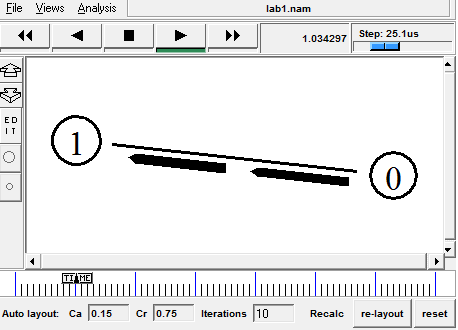
\includegraphics[width=0.40\textwidth]{1.png}
\end{figure}
\newpage
\item Ποια είναι η απάντησή σας στο προηγούμενο ερώτημα, αν διπλασιαστεί η καθυστέρηση της ζεύξης;
Επιβεβαιώστε την απάντησή σας από το \textlatin{animation.}\\
 \textbf{Απάντηση} : Όταν έχουμε καθυστέρηση ζεύξης 10 $msec$ είδαμε ότι έχουμε 2 πακέτα στη ζεύξη. Τώρα διπλασιάζοντας την καθυστέρηση ζεύξης , θα έχουμε $2*2=4$ πακέτα, άρα συνολικά : 4000 $bytes$.Παρακάτω, φαίνεται και στο \textlatin{animation}.
 \begin{figure}[htbp]
	 \centering
		 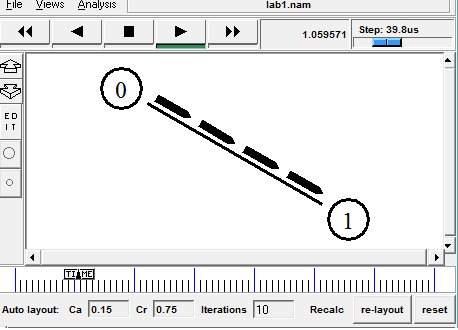
\includegraphics[width=0.45\textwidth]{2.png}
 \end{figure}
\item Εάν υποθέσουμε ότι σε κάθε πακέτο οι επικεφαλίδες του $IP$ και του $UDP$ μαζί έχουν μήκος 40 $byte$,
ποιος είναι ο καθαρός ρυθμός μετάδοσης των δεδομένων σε $bit/sec?$\\
\textbf{Απάντηση} : Πλέον τα καθαρά δεδομένα μας είναι $1000-40=960$ \textlatin{bytes}. Άρα, ο νέος ρυθμός μετάδοσης είναι : $\frac{8*960}{0.005}=1.536.000$ \textlatin{bits}.
\item Ποιες παράμετροι μπορεί να αλλαχθούν για να μεταβληθεί ο ρυθμός μετάδοσης και με ποιες εντολές
επιτυγχάνονται αυτές οι αλλαγές\textlatin{?}\\
\textbf{Απάντηση} : Ο ρυθμός μετάδοσης επηρεάζεται από το μέγεθος του πακέτου , καθώς και από το ρυθμό μετάδοσης του πακέτου. Αυτές οι παράμετροι καθορίζονται από τις παρακάτω εντολές : \\
\selectlanguage{english}
\begin{lstlisting}
$traffic0 set packetSize_SIZE
$traffic0 set interval_INTERVAL 
\end{lstlisting}
\selectlanguage{greek}
\item Αν επιθυμούμε να έχουμε καθαρό ρυθμό μετάδοσης δεδομένων ίσο με $1.2 Mbit/sec$, μεταβάλλοντας
κάθε φορά μία από τις ανωτέρω παραμέτρους, ποιες τιμές προτείνετε για κάθε μία; Ελέγξτε κάθε
φορά αν οι απαντήσεις σας δίνουν ρυθμό μετάδοσης μικρότερο από τη χωρητικότητα της ζεύξης.\\
\textbf{Απάντηση} :Θεωρούμε πως οι τιμές για τους $IP$ και $UDP$ που υποθέσαμε στο παραπάνω ερώτημα είναι ίδιες. Κρατώντας σταθερό το $interval$ θα πρέπει να μεταβάλλουμε το μέγεθος του πακέτου ως εξής : $\frac{1.2*10^6*0.005}{8}+40 = 790 $ \textlatin{bytes}. Κρατώντας σταθερό το μέγεθος του πακέτου , θα πρέπει να μεταβάλλουμε το ρυθμό μετάδοσης των πακέτων ως εξής : $\frac{8*960}{1.2*10^6}=0.0064$ \textlatin{sec}.Βλέπουμε πως και για τις δύο τιμές δεν υπερβαίνουμε τη χωρητικότητα της ζεύξης.
\item Για ποιες τιμές των ανωτέρω παραμέτρων θα αρχίσει να παρατηρείται οριακά η απώλεια πακέτων;
Επιβεβαιώστε την απάντησή σας τρέχοντας το \textlatin{tcl script} και το \textlatin{animation}.\\ 
\textbf{Απάντηση} : Για να έχουμε απώλεια πακέτων θα πρέπει ο ρυθμός μετάδοσης των δεδομένων να υπερβαίνει το εύρος ζώνης της ζεύξης. Οπότε, στη συγκεκριμένη περίπτωση οριακά θα έχουμε απώλεια δεδομένων για ρυθμό μετάδοσης ίσο με $2 Mb/s$.Άρα, κρατώντας σταθερό, αρχικά το μέγεθος του πακέτου και ύστερα το ρυθμό μετάδοσης των πακέτων βρίσκουμε αντίστοιχα : $interval= \frac{1000*8}{2*10^6}=0.004 $ \textlatin{sec} και μέγεθος πακέτου $=1250$ \textlatin{bytes}.\\\\

\end{itemize}
\textbf{{\underline{2.Μελέτη τοπολογίας με το \textlatin{Xgraph} }}}  \\Στην άσκηση αυτή χρησιμοποιούμε το \textlatin{Xgraph} για να δημιουργήσουμε γραφικές παραστάσεις της κίνησης στο δίκτυο που ήδη μελετάμε.Εκτελώντας τον κώδικα με τα συγκεκριμένα δεδομένα προκύπτει το παρακάτω διάγραμμα :
\begin{figure}[htbp]
	\centering
		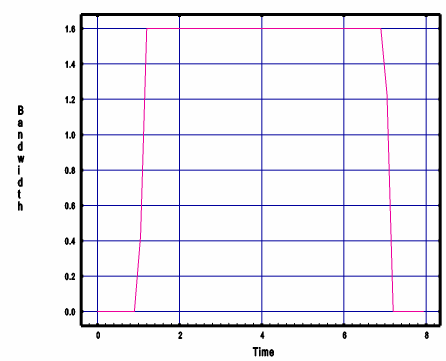
\includegraphics[width=0.50\textwidth]{3.png}
\end{figure}
Βλέπουμε, ότι επιβεβαιώνεται ο ρυθμός μετάδοσης των δεδομένων στα 1.600.000 \textlatin{bits/sec} που βρήκαμε στην αρχή.\\\\

\textsl{\textbf{Απαντήσεις ερωτήσεων}}
\begin{itemize}
	\item Μεταβάλλοντας την τιμή του μήκους του πακέτου διαπιστώστε και σχολιάστε πώς μεταβάλλεται η
γραφική παράσταση της μεταφερόμενης κίνησης. \\
\textbf{Απάντηση} : Εφόσον τα δύο μεγέθη είναι γραμμικώς ανάλογα, αν αυξήσουμε το μέγεθος του πακέτου θα αυξηθεί και το ύψος της γραφικής, ενώ αν μειώσουμε το μέγεθος του πακέτου , θα μειωθεί και το ύψος της γραμμής. Αν αυξήσουμε το μέγεθος του πακέτου σε άνω των 1250 $bytes$ (για το οποίο έχουμε οριακά απώλειες όπως είδαμε) θα παρατηρήσουμε ψαλιδισμό.
\item Ποιο είναι το μέγιστο μήκος πακέτου που μπορεί να αποσταλεί χωρίς να ξεπερνάται η
χωρητικότητα της γραμμής; \\
\textbf{Απάντηση} : Η απάντηση είναι παρόμοια με την παραπάνω. Το μέγιστο μήκος του πακέτου είναι 1250 $bytes$ , καθώς όπως βλέπουμε και διαγραμματικά όσο απομακρυνόμαστε από αυτό το όριο , τόσο μεγαλύτερος ο ψαλιδισμός.Πχ για μέγεθος πακέτου 1400 $bytes$ φαίνεται παρακάτω ο ψαλιδισμός:
\begin{figure}[htbp]
	\centering
		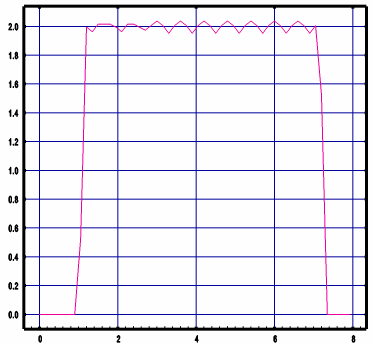
\includegraphics[width=0.50\textwidth]{4.png}
\end{figure}
\item Διατηρώντας σταθερό το μήκος πακέτου, μεταβάλλετε τον ρυθμό μετάδοσης. Τι παρατηρείτε στη
γραφική παράσταση της μεταφερόμενης κίνησης και πώς το ερμηνεύετε; \\
\textbf{Απάντηση} : Το να μεταβάλουμε τον ρυθμό μετάδοσης διατηρώντας σταθερό το μήκος του πακέτου , σημαίνει πως μεταβάλλουμε το ρυθμό μετάδοσης των πακέτων.Τα δύο αυτά μεγέθη είναι αντιστρόφως ανάλογα.Άρα, όσο μειώνουμε το ρυθμό μετάδοσης των πακέτων μεγαλώνει ο ρυθμός μετάδοσης μέχρι να ξεπεράσουμε τη χωρητικότητα της ζεύξης και να προκληθεί ψαλιδισμός.

\item Αυξήστε την καθυστέρηση της γραμμής σύνδεσης των δυο κόμβων σε 0.5 δευτερόλεπτα. Τι
παρατηρείτε στην γραφική παράσταση της μεταφερόμενης κίνησης; Επαναφέρετε την καθυστέρηση
στην αρχική τιμή. \\
\textbf{Απάντηση} : Από το διάγραμμα,φαίνεται ότι η γραφική παράσταση μετατίθεται κατά 0.5 δευτερόλεπτα δεξιά. Αυτό οφείλεται στο ότι η καταγραφή γίνεται στον υποδοχέα και συνεπώς , υφίσταται την καθυστέρηση της ζεύξης:
\begin{figure}[htbp]
	\centering
		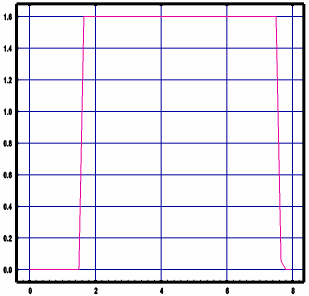
\includegraphics[width=0.30\textwidth]{5.png}
\end{figure}

\item Πώς επηρεάζει τη γραφική παράσταση ο χρόνος που επαναλαμβάνεται η διαδικασία “$record$”.
Προτείνετε έναν κατάλληλο χρόνο για να επιτύχετε μια γραφική παράσταση στιγμιαίας κίνησης και
μια μέσης\\
\textbf{Απάντηση} : Βλέπουμε από το διάγραμμα ότι αυξομειώνοντας αυτό το χρόνο , μεταβάλλουμε την κλίση των καθέτων της γραφικής παράστασης, δηλαδή μεταβάλλουμε το πόσο απότομη είναι η γραφική παράσταση.Πρακτικα΄,  ο χρόνος αυτός καθορίζει την ταχύτητα που το πρόγραμμα λαμβάνει στιγμιότυπα της προσομοίωσης. Αν θέλουμε στιγμιαία κίνηση θα επιλέξουμε ένα μικρό χρόνο, όπως πχ 0.01 $sec$.Για τη μέση κίνηση θα επιλέξουμε ένα μεγάλο χρόνο επαναληψιμότητας, όπως πχ 1.0 $sec$.  
\item Η κίνηση μεταξύ των δυο κόμβων είναι σταθερής ροής ($CBR$). Αλλάξτε την κίνηση σε εκθετική
θέτοντας “$Exponential$” όπου υπάρχει “$CBR$”. Εξηγήστε τη γραφική παράσταση της κίνησης. Για να
βγάλετε σωστά συμπεράσματα, θα πρέπει να αυξήσετε τον χρόνο αποστολής της κίνησης, και
φυσικά της προσομοίωσης, τουλάχιστον σε 20 δευτερόλεπτα και να ξανατρέξετε το $script$.\\ 
\textbf{Απάντηση} : Παρακάτω φαίνεται η γραφική παράσταση με εκθετική κίνηση δεδομένων.(η δεύτερη είναι σε μικρότερο χρόνο προσομοιώσης , άλλα και με μικρότερο χρόνο λήψης στιγμιοτύπων για μεγαλύτερη ακρίβεια). Η μορφή αυτή οφείλεται στό ότι ο χρόνος κάθε περιόδου υπολογίζεται απο εκθετικές συναρτήσεις, ενώ με $CBR$ υπολογίζεται με ομοιόμορφες συναρτήσεις.

\begin{figure}[htbp]
	\centering
		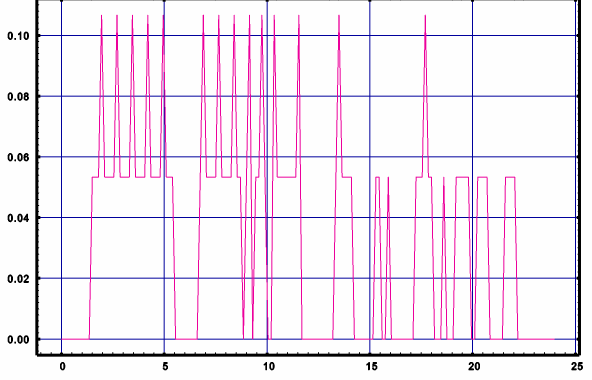
\includegraphics[width=0.45\textwidth]{6.png}
	\caption{χρόνος λήψης στιγμιοτύπων= 0.15 δευτερόλεπτα}
\end{figure}
\begin{figure}[htbp]
	\centering
	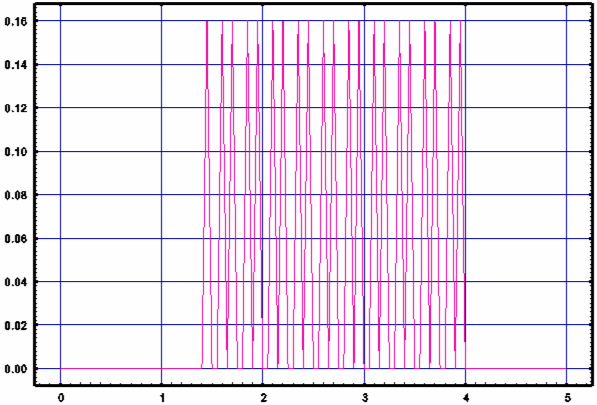
\includegraphics[width=0.45\textwidth]{7.png}
	\caption{χρόνος λήψης στιγμιοτύπων= 0.05 δευτερόλεπτα}
\end{figure}


\end{itemize}

Τέλος , ακολουθεί ο κώδικας που εκτελέστηκε στον $NS2$ $simulator$  για την ζεύξη των δύο κόμβων με εκθετική συνάρτηση χρόνου λήψης.\\\\

\selectlanguage{english}

\begin{lstlisting}

set ns [new Simulator]
set nf [open lab1.nam w]
$ns namtrace-all $nf
set xf [open lab1.tr w]
proc record {} {
 global sink xf
 set ns [Simulator instance]
 set time 0.05
 set bw [$sink set bytes_]
 set now [$ns now]
 puts $xf "$now [expr ((($bw/$time)*8)/1000000)]"
 $sink set bytes_ 0
 $ns at [expr $now+$time] "record"
}
proc finish {} {
 global ns nf xf
 $ns flush-trace
 close $nf
 close $xf
 exit 0
}
set n0 [$ns node]
set n1 [$ns node]
$ns duplex-link $n0 $n1 2Mb 10ms DropTail
set agent0 [new Agent/UDP]
$agent0 set packetSize_ 1000
$ns attach-agent $n0 $agent0
set traffic0 [new Application/Traffic/Exponential]
$traffic0 set packetSize_ 1000
$traffic0 set interval_ 0.005
$traffic0 attach-agent $agent0
set sink [new Agent/LossMonitor]
$ns attach-agent $n1 $sink
$ns connect $agent0 $sink 
$ns at 0.0 "record"
$ns at 1.0 "$traffic0 start"
$ns at 4.0 "$traffic0 stop"
$ns at 5.0 "finish"
$ns run

\end{lstlisting}




\end{document}
